

\tikzset{every picture/.style={line width=0.75pt}} %set default line width to 0.75pt        

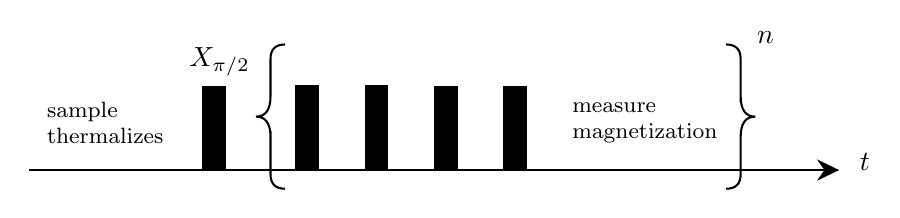
\begin{tikzpicture}[x=0.75pt,y=0.75pt,yscale=-1,xscale=1]
%uncomment if require: \path (0,300); %set diagram left start at 0, and has height of 300

%Straight Lines [id:da3553357763402164] 
\draw    (7,139.5) -- (394.5,139.5) ;
\draw [shift={(397.5,139.5)}, rotate = 180] [fill={rgb, 255:red, 0; green, 0; blue, 0 }  ][line width=0.08]  [draw opacity=0] (10.72,-5.15) -- (0,0) -- (10.72,5.15) -- (7.12,0) -- cycle    ;
%Shape: Rectangle [id:dp9462927331579177] 
\draw  [fill={rgb, 255:red, 0; green, 0; blue, 0 }  ,fill opacity=1 ] (91,99.5) -- (101.5,99.5) -- (101.5,139.5) -- (91,139.5) -- cycle ;
%Shape: Brace [id:dp5361701357698033] 
\draw   (130.5,79) .. controls (125.83,79) and (123.5,81.33) .. (123.5,86) -- (123.5,103.75) .. controls (123.5,110.42) and (121.17,113.75) .. (116.5,113.75) .. controls (121.17,113.75) and (123.5,117.08) .. (123.5,123.75)(123.5,120.75) -- (123.5,141.5) .. controls (123.5,146.17) and (125.83,148.5) .. (130.5,148.5) ;
%Shape: Brace [id:dp6964209405349638] 
\draw   (343,148.5) .. controls (347.67,148.5) and (350,146.17) .. (350,141.5) -- (350,123.75) .. controls (350,117.08) and (352.33,113.75) .. (357,113.75) .. controls (352.33,113.75) and (350,110.42) .. (350,103.75)(350,106.75) -- (350,86) .. controls (350,81.33) and (347.67,79) .. (343,79) ;
%Shape: Rectangle [id:dp10957639024886712] 
\draw  [fill={rgb, 255:red, 0; green, 0; blue, 0 }  ,fill opacity=1 ] (136,99) -- (146.5,99) -- (146.5,139) -- (136,139) -- cycle ;
%Shape: Rectangle [id:dp4589647059466161] 
\draw  [fill={rgb, 255:red, 0; green, 0; blue, 0 }  ,fill opacity=1 ] (169.33,99) -- (179.83,99) -- (179.83,139) -- (169.33,139) -- cycle ;
%Shape: Rectangle [id:dp07946714725560555] 
\draw  [fill={rgb, 255:red, 0; green, 0; blue, 0 }  ,fill opacity=1 ] (202.66,99.5) -- (213.16,99.5) -- (213.16,139.5) -- (202.66,139.5) -- cycle ;
%Shape: Rectangle [id:dp016286675726323585] 
\draw  [fill={rgb, 255:red, 0; green, 0; blue, 0 }  ,fill opacity=1 ] (236,99.5) -- (246.5,99.5) -- (246.5,139.5) -- (236,139.5) -- cycle ;

% Text Node
\draw (406,129.9) node [anchor=north west][inner sep=0.75pt]    {$t$};
% Text Node
\draw (98.94,87.19) node    {$X_{\pi /2}$};
% Text Node
\draw (43.87,116.75) node  [font=\footnotesize] [align=left] {sample\\thermalizes};
% Text Node
\draw (356.5,71.4) node [anchor=north west][inner sep=0.75pt]    {$n$};
% Text Node
\draw (303.87,116.75) node  [font=\footnotesize] [align=left] {measure\\magnetization};


\end{tikzpicture}
